\textbf{2-1}. 如本题图所示,一条无穷长直导线在一处弯折成 $1/4$ 圆弧,圆弧的半径为 $R$，圆心在 $O$，直线的延长线都通过圆心。已知导线中的电流为 $I$，求 $O$ 点的磁感应强度。

\begin{center}
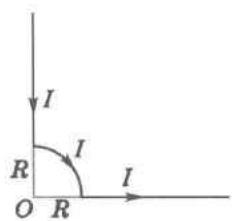
\includegraphics[width=0.2\linewidth]{figures/习题2-1.jpg}
\end{center}

\vfill


\textbf{2-2.} 如本题图所示, 两条无穷长的平行直导线相距为 $2a$ , 分别载有方向相同的电流 $I_{1}$ 和 $I_{2}$ . 空间任一点 $P$ 到 $I_{1}$ 的垂直距离为 $x_{1}$ 、到 $I_{2}$ 的垂直距离为 $x_{2}$ , 求 $P$ 点的磁感应强度 $\pmb{B}$ .

\begin{center}
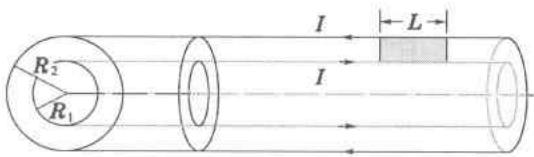
\includegraphics[width=0.4\linewidth]{figures/习题2-2.jpg}
\end{center}

\vfill\newpage

\textbf{2-3.} 如本题图所示, 两条无穷长的平行直导线相距为 $2a$ , 载有大小相等而方向相反的电流 $I$ . 空间任一点 $P$ 到两导线的垂直距离分别为 $x_{1}$ 和 $x_{2}$ , 求 $P$ 点的磁感应强度 $\pmb{B}$ .
\begin{center}
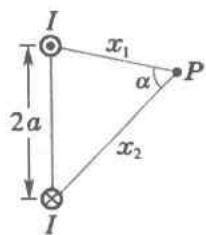
\includegraphics[width=0.2\linewidth]{figures/习题2-3.jpg}
\end{center}

\vfill


\textbf{2-4.} 如本题图, 两条无限长直载流导线垂直而不相交, 其间最近距离为 $d = 2.0 \mathrm{~cm}$ , 电流分别为 $I_{1} = 4.0 \mathrm{~A}$ 和 $I_{2} = 6.0 \mathrm{~A}$ . $P$ 点到两导线的距离都是 $d$ , 求 $P$ 点的磁感应强度 $\pmb{B}$ .
\begin{center}
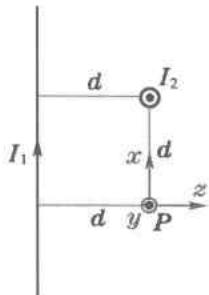
\includegraphics[width=0.3\linewidth]{figures/习题2-4a.jpg}
\end{center}


\vfill\newpage

\textbf{2-5.} 载流等边三角形线圈边长为 $2a$ ，电流为 $I$

(1) 求轴线上距中心为 $r_{0}$ 处的磁感应强度。

(2) 证明：当 $r_{0} \gg a$ 时轴线上磁感应强度具有如下形式：
$$
B = \frac {\mu_ {0} m}{2 \pi r _ {0} ^ {3}},
$$
式中 m=IS 为三角形线圈的磁矩。

\vfill


\textbf{2-6.} 电流均匀地流过宽为 $2a$ 的无穷长平面导体薄板。电流大小为 $I$ ，通过板的中线并与板面垂直的平面上有一点 $P, P$ 到板的垂直距离为 $x$ （见本题图），设板厚可略去不计。
(1) 求 P 点的磁感应强度 B.
(2) 当 $a \to \infty$ ，但 $\iota = I/2a$ （单位宽度上的电流，叫做面电流密度）为一常量时 P 点的磁感应强度。
\begin{center}
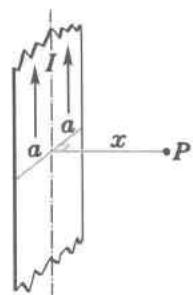
\includegraphics[width=0.2\linewidth]{figures/习题2-6.jpg}
\end{center}

\vfill\newpage

\textbf{2-7.} 如本题图, 两无穷大平行平面上都有均匀分布的面电流, 面电流密度 (见上题) 分别为 $\iota_{1}$ 和 $\iota_{2}$ , 两电流平行。求:

(1) 两面之间的磁感应强度；

(2) 两面之外空间的磁感应强度；

(3) $\iota_{1}=\iota_{2}=\iota$ 时结果如何?

(4) 在情形(3)中电流反平行, 情形如何?

(5) 在情形(3)中电流方向垂直, 情形如何?

\vfill


\textbf{2-8.} 半径为 $R$ 的无限长直圆筒上有一层均匀分布的面电流，电流都环绕着轴线流动并与轴线方向成一角度 $\theta$ ，即电流在筒面上沿螺旋线向前流动（见本题图）。设面电流密度为 $\iota$ ，求轴线上的磁感应强度。
\begin{center}
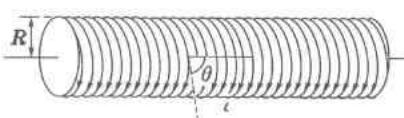
\includegraphics[width=0.4\linewidth]{figures/习题2-8.jpg}
\end{center}


\vfill\newpage

\textbf{2-9.} 一很长的螺线管，由外皮绝缘的细导线密绕而成，每厘米有35匝。当导线中通过的电流为 $2.0\mathrm{A}$ 时，求这螺线管轴线上中心和端点的磁感强应强度。

\vfill


\textbf{2-11.} 用直径 $0.163\mathrm{cm}$ 的铜线绕在 $6.0\mathrm{cm}$ 直径的圆筒上，做成一个单层螺线管。管长 $30\mathrm{cm}$ ，每厘米绕5匝。铜线在 $75^{\circ}\mathrm{C}$ 时每米电阻 $0.010\Omega$ （假设通电后导线将达此温度）。将此螺线管接在 $2.0\mathrm{V}$ 的蓄电池上，其中磁感应强度和功率消耗各多少？

\vfill\newpage

\textbf{2-12.} 球形线圈由表面绝缘的细导线在半径为 $R$ 的球面上密绕而成，线圈的中心都在同一直径上，沿这直径单位长度内的匝数为 $n$ ，并且各处的 $n$ 都相同，通过线圈的电流为 $I$ 。设该直径上一点 $P$ 到球心的距离为 $x$ ，求下列各处的磁感应强度 $B$ ：

(1) $x = 0$ （球心）；

(2) $x=R$ (该直径与球面的交点);

(3) $x < R$ (球内该直径上任一点);

(4) $x > R$ （球外该直径上任一点）。

\vfill


\textbf{2-13.} 半径为 $R$ 的球面上均匀分布着电荷，面密度为 $\sigma_{\mathrm{e}}$ 。当这球面以角速度 $\omega$ 绕它的直径旋转时，求转轴上球内和球外任一点的磁感应强度分布。

\vfill\newpage

\textbf{2-14.} 半径为 $R$ 的圆片上均匀带电，面密度为 $\sigma_{\mathrm{e}}$ 。令该片以匀角速度 $\omega$ 绕它的轴旋转，求轴线上距圆片中心 $O$ 为 $x$ 处的磁场（见本题图）。
\begin{center}
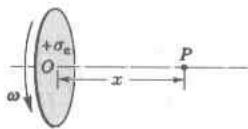
\includegraphics[width=0.4\linewidth]{figures/习题2-14.jpg}
\end{center}

\vfill


\textbf{2-15.} 氢原子处在正常状态(基态)时,它的电子可看作是在半径为 $a=0.53\times10^{-8}cm$ 的轨道(叫做玻尔轨道)上作匀速圆周运动,速率为 $v=2.2\times10^{8}cm/s$ . 已知电子电荷的大小为 $e=1.6\times10^{-19}C$ ,求电子的这种运动在轨道中心产生的磁感强度B的值。

\vfill\newpage

\textbf{2-16.} 一载有电流 $I$ 的无穷长直空心圆筒，半径为 $R$ （筒壁厚度可以忽略），电流沿它的轴线方向流动，并且是均匀分布的，分别求离轴线为 $r < R$ 和 $r > R$ 处的磁场。

\vfill


\textbf{2-17.} 有一很长的载流导体直圆管，内半径为 $a$ ，外半径为 $b$ ，电流为 $I$ ，电流沿轴线方向流动，并且均匀分布在管壁的横截面上（见本题图）。空
\begin{center}
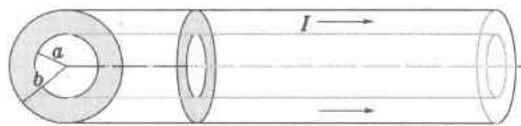
\includegraphics[width=0.5\linewidth]{figures/习题2-17.jpg}
\end{center}
间某一点到管轴的垂直距离为 $r$，求：
(1) $r<a$，
(2) $a<r<b$，
(3) $r>b$ 等处的磁感应强度。

\vfill\newpage

\textbf{2-18.} 一很长的导体直圆管，管厚为 $5.0\mathrm{mm}$ ，外直径为 $50\mathrm{mm}$ ，载有50A的直流电，电流沿轴向流动，并且均匀分布在管的横截面上。求下列几处磁感应强度的大小 $B$ ：

(1) 管外靠近外壁；

(2) 管内靠近内壁；

(3) 内外壁之间的中点。

\vfill


\textbf{2-19.} 电缆由一导体圆柱和一同轴的导体圆筒构成。使用时，电流 $I$ 从一导体流去，从另一导体流回，电流都均匀分布在横截面上。设圆柱的半径为 $r_1$ ，圆筒的内外半径分别为 $r_2$ 和 $r_3$ （见本题图）， $r$ 为到轴线的垂直距离，求 $r$ 从 $0$ 到 $\infty$ 的范围内各处的磁感应强度 $B$ .
\begin{center}
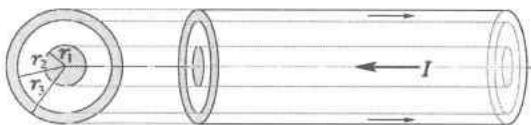
\includegraphics[width=0.5\linewidth]{figures/习题2-19.jpg}
\end{center}

\vfill\newpage

\textbf{2-20.} 一对同轴无穷长直的空心导体圆筒，内、外筒半径分别为 $R_{1}$ 和 $R_{2}$ （筒壁厚度可以忽略）。电流 $I$ 沿内筒流去，沿外筒流回（见本题图），

(1) 计算两筒间的磁感应强度 $B$;

(2) 通过长度为 $L$ 的一段截面(图中阴影区)的磁通量 $\Phi_{B}$ ;

(3) 计算磁矢势 $A$ 在两筒间的分布。

\begin{center}
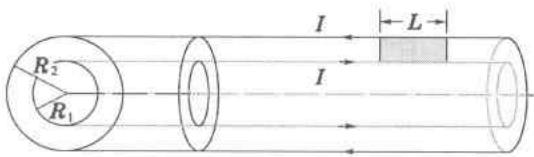
\includegraphics[width=0.5\linewidth]{figures/习题2-20.jpg}
\end{center}

\vfill


\textbf{2-21.} 矩形截面的螺绕环，尺寸见本题图。
(1) 求环内磁感应强度的分布；
(2) 证明通过螺绕环截面(图中阴影区)的磁通量为 $\Phi_{B}=\frac{\mu_{0}NIh}{2\pi}\ln\frac{D_{1}}{D_{2}}$
其中 N 为螺绕环总匝数，I 为其中电流的大小。
\begin{center}
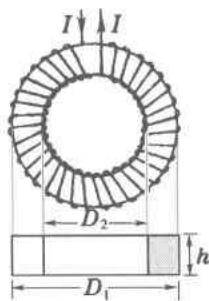
\includegraphics[width=0.2\linewidth]{figures/习题2-21.jpg}
\end{center}

\vfill\newpage

\textbf{2-22.} 用安培环路定理重新计算习题2-6(2)中无限大均匀载流平面外的磁感应强度。

\vfill


\textbf{2-23.} 如本题图所示,有一根长为 $l$ 的直导线,质量为 $m$ ,用细绳子平挂在外磁场 $\pmb{B}$ 中,导线中通有电流 $I,I$ 的方向与 $\pmb{B}$ 垂直。

(1) 求绳子张力为 0 时的电流 I. 当 $l = 50 \, cm$ , $m = 10 \, g$ , B = 1.0 T 时, I = ?

(2) 在什么条件下导线会向上运动?
\begin{center}
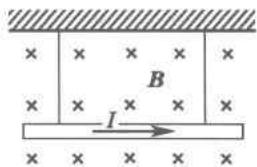
\includegraphics[width=0.4\linewidth]{figures/习题2-23.jpg}
\end{center}


\vfill\newpage

\textbf{2-24.} 横截面积 $S = 2.0\mathrm{mm}^2$ 的铜线弯成如本题图中所示形状，其中 $OA$ 和 $DO'$ 段固定在水平方向不动，ABCD段是边长为 $a$ 的正方形的三边，可以绕 $OO'$ 转动；整个导线放在均匀磁场 $\pmb{B}$ 中， $\pmb{B}$ 的方向竖直向上。已知铜的密度 $\rho=8.9g/cm^{3}$ ，当这铜线中的 I=10A 时，在平衡情况下，AB 段和 CD 段与竖直方向的夹角 $\alpha=15^{\circ}$ ，求磁感应强度 B 的大小。
\begin{center}
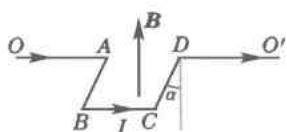
\includegraphics[width=0.5\linewidth]{figures/习题2-24.jpg}
\end{center}


\vfill


\textbf{2-25.} 一段导线弯成如本题图中所示的形状, 它的质量为 $m$ , 上面水平一段的长度为 $l$ , 处在均匀磁场中, 磁感应强度为 $\pmb{B}, \pmb{B}$ 与导线垂直; 导线下面两端分别插在两个浅水银槽里, 两槽水银与一带开关 $\mathbf{K}$ 的外电源连接。当 $\mathbf{K}$ 一接通, 导线便从水银槽里跳起来。


(1) 设跳起来的高度为 h, 求通过导线的电量 q;

(2) 当 $m = 10 \, g, l = 20 \, cm, h = 3.0 \, m, B = 0.10 \, T$ 时，求 q 的量值。
\begin{center}
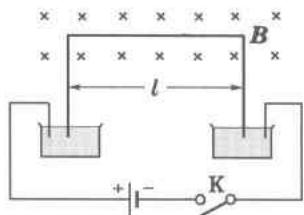
\includegraphics[width=0.4\linewidth]{figures/习题2-25.jpg}
\end{center}
\vfill\newpage

\textbf{2-26.} 安培秤如本题图所示,它的一臂下面挂有一个矩形线圈,线圈共有 $N$ 匝,线圈的下部悬挂在均匀磁场 $\pmb{B}$ 内,下边一段长为 $l$ ,它与 $\pmb{B}$ 垂直。当线圈的导线中通有电流 $I$ 时,调节砝码使两臂达到平衡;然后使电流反向,这时需要在一臂上加质量为 $m$ 的砝码,才能使两臂再达到平衡。

(1) 求磁感应强度 B 的大小 B;

(2) 当 N=9, l=10.0 cm, I=0.100 A, m=8.78 g 时, 设 $g=9.80\ m/s^{2}$ , B=?

\vfill


\textbf{2-27.} 一矩形载流线圈由20匝互相绝缘的细导线绕成，矩形边长为 $10.0\mathrm{cm}$ 和 $5.0\mathrm{cm}$ ，导线中的电流为 $0.10\mathrm{A}$ ，这线圈可以绕它的一边 $OO'$ 转动（见本题图）。当加上 $B = 0.50\mathrm{T}$ 的均匀外磁场、 $B$ 与线圈平面成 $30^{\circ}$ 角时，求这线圈受到的力矩。

\vfill\newpage

\textbf{2-28.} 一边长为 $a$ 的正方形线圈载有电流 $I$ , 处在均匀外磁场 $\pmb{B}$ 中, $\pmb{B}$ 沿水平方向,线圈可以绕通过中心的竖直轴 $OO'$ 转动（见本题图）,转动惯量为 J. 求线圈在平衡位置附近作微小摆动的周期 T.

\vfill


\textbf{2-29.} 一螺线管长 $30\mathrm{cm}$ , 横截面的直径为 $15\mathrm{mm}$ , 由表面绝缘的细导线密绕而成, 每厘米绕有 100 匝。当导线中通有 $2.0\mathrm{A}$ 的电流后, 把这螺线管放到 $B = 4.0\mathrm{T}$ 的均匀磁场中, 求:

(1) 螺线管的磁矩；

(2) 螺线管所受力矩的最大值。

\vfill\newpage

\textbf{2-30.} 两条很长的平行输电线相距 $20\mathrm{mm}$ ，都载有 $100\mathrm{A}$ 的电流，分别求电流方向相同和相反时，其中两段 $1\mathrm{m}$ 长的输电线之间的相互作用力。

\vfill


\textbf{2-31.} 发电厂的汇流条是两条 $3\mathrm{m}$ 长的平行铜棒，相距 $50\mathrm{cm}$ ；当向外输电时，每条棒中的电流都是 $10000\mathrm{A}$ 。作为近似，把两棒当作无穷长的细线，试计算它们之间的相互作用力。

\vfill\newpage

\textbf{2-32.} 载有电流 $I_{1}$ 的长直导线旁边有一正方形线圈，边长为 $2a$ ，载有电流 $I_{2}$ ，线圈中心到导线的垂直距离为 $b$ ，电流方向如本题图所示。线圈可以绕平行于导线的轴 $O_{1}O_{2}$ 转动。求：

(1) 线圈在 $\theta$ 角度位置时所受的合力 F 和合力矩 L;

(2) 线圈平衡时 $\theta$ 的值；

(3) 线圈从平衡位置转到 $\theta = \pi / 2$ 时， $I_{1}$ 作用在线圈上的力作了多少功？
\begin{center}
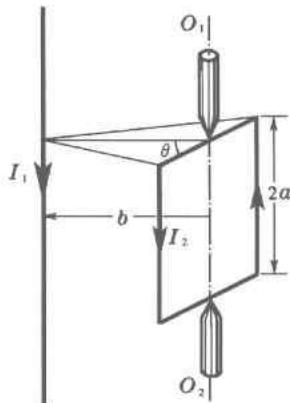
\includegraphics[width=0.2\linewidth]{figures/习题2-32.jpg}
\end{center}

\vfill


\textbf{2-33.} 载有电流 $I_{1}$ 的长直导线旁边有一平面圆形线圈，线圈半径为 $r$ ，中心到直导线的距离为 $l$ ，线圈载有电流 $I_{2}$ ，线圈和直导线在同一平面内（见本题图）。求 $I_{1}$ 作用在圆形线圈上的力。
\begin{center}
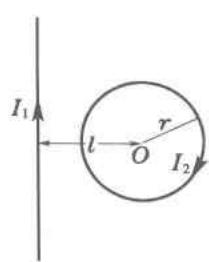
\includegraphics[width=0.2\linewidth]{figures/习题2-33.jpg}
\end{center}

\vfill\newpage

\textbf{2-34.} 试证明电子绕原子核沿圆形轨道运动时磁矩与角动量大小之比为
$$
\gamma = \frac {- e}{2 m} (\text { 经典回旋磁比率 }),
$$
式中 $-e$ 和 $m$ 是电子的电荷与质量，负号表示磁矩与角动量的方向相反，如图。（它们各沿什么方向？）
【提示：计算磁矩时，可把在圆周上运动的电子看成是电流环。】
\begin{center}
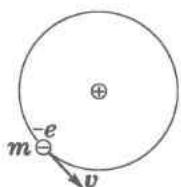
\includegraphics[width=0.2\linewidth]{figures/习题2-34.jpg}
\end{center}


\vfill


\textbf{2-35.} 一磁电式电流计线圈长 $a = 2.0\mathrm{cm}$ , 宽 $b = 1.0\mathrm{cm}$ , $N = 250$ 匝, 磁极间隙内的磁感应强度 $B = 2000\mathrm{Gs}$ . 当通入电流 $I = 0.10\mathrm{mA}$ 时, 偏转角 $\theta = 30^{\circ}$ , 求:

(1) 作用在线圈上的磁偏转力矩 $L_{磁}$ ;

(2) 游丝的扭转常数 D.

\vfill\newpage

\textbf{2-36.} 带电粒子穿过过饱和蒸气时，在它走过的路径上，过饱和蒸气便凝结成小液滴，从而使得它运动的轨迹（径迹）显示出来，这就是云室的原理。今在云室中有 $B = 10000\mathrm{Gs}$ 的均匀磁场，观测到一个质子的径迹是圆弧, 半径 $r=20\,cm$ , 已知这粒子的电荷为 $1.6\times10^{-19}\,C$ , 质量为 $1.67\times10^{-27}\,kg$ , 求它的动能。

\vfill


\textbf{2-37.} 测得一太阳黑子的磁场为 $B = 4000\mathrm{Gs}$ ，问其中电子以(1) $5.0\times 10^{7}\mathrm{cm / s}$ ，(2) $5.0\times 10^{8}\mathrm{cm / s}$ 的速度垂直于 $\pmb{B}$ 运动时，受到的洛伦兹力各有多大？回旋半径各有多大？已知电子电荷的大小为 $1.6\times 10^{-19}\mathrm{C}$ ，质量为 $9.1\times 10^{-31}\mathrm{kg}$ .

\vfill\newpage

\textbf{2-38.} 一电子以 $v = 3.0 \times 10^{7} \, \text{m/s}$ 的速率射入匀强磁场 $B$ 内，它的速度与 $B$ 垂直， $B = 10 \, \text{T}$ . 已知电子电荷 $-e = -1.6 \times 10^{-19} \, \text{C}$ ，质量 $m = 9.1 \times 10^{-31} \, \text{kg}$ ，求这电子所受的洛伦兹力，并与它在地面所受的重力加以比较。

\vfill


\textbf{2-39.} 已知质子质量 $m = 1.67 \times 10^{-27} \mathrm{~kg}$ , 电荷 $e = 1.6 \times 10^{-19} \mathrm{C}$ , 地球半径 $6370 \mathrm{~km}$ , 地球赤道上地面的磁场 $B = 0.32 \mathrm{Gs}$ .

(1) 要使质子绕赤道表面作圆周运动, 其动量 p 和能量 E 应有多大?

(2) 若要使质子以速率 $v = 1.0 \times 10^{7} \, m/s$ 环绕赤道表面作圆周运动, 问地磁场应该有多大?
【提示:相对论中粒子的动量p和能量E的公式如下:
$$
\begin{array}{c} {\pmb {p} = m \pmb {v},} \\ {E = m c ^ {2} = c \sqrt {p ^ {2} + m _ {0} ^ {2} c ^ {2}},} \end{array}
$$
m 和 $m_{0}$ 的关系为：
$$
m = \frac {m _ {0}}{\sqrt {1 - v ^ {2} / c ^ {2}}}.
$$】


\vfill\newpage

\textbf{2-40.} 在一个显像管里，电子沿水平方向从南到北运动，动能是 $1.2 \times 10^{4} \mathrm{eV}$ 。该处地球磁场在竖直方向上的分量向下， $B$ 的大小是 0.55Gs。已知电子电荷 $-e = -1.6 \times 10^{-19} \mathrm{C}$ ，质量 $m = 9.1 \times 10^{-31} \mathrm{~kg}$ 。

(1) 电子受地磁的影响往哪个方向偏转?

(2) 电子的加速度有多大?

(3) 电子在显像管内走 20 cm 时, 偏转有多大?

(4) 地磁对看电视有没有影响?

\vfill


\textbf{2-41.} 如本题图所示，一质量为 $m$ 的粒子带有电量 $q$ ，以速度 $v$ 射入磁感应强度为 $B$ 的均匀磁场， $v$ 与 $B$ 垂直；粒子从磁场出来后继续前进。已知磁场区域在 $v$ 方向（即 $x$ 方向）上的宽度为 l，当粒子从磁场出来后在 x 方向前进的距离为 L-l/2 时，求它的偏转 y.
\begin{center}
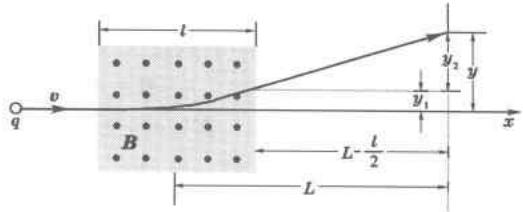
\includegraphics[width=0.4\linewidth]{figures/习题2-41.jpg}
\end{center}


\vfill\newpage

\textbf{2-42.} 一氘核在 $B = 1.5\mathrm{T}$ 的均匀磁场中运动，轨迹是半径为 $40\mathrm{cm}$ 的圆周。已知氘核的质量为 $3.34 \times 10^{-27}\mathrm{kg}$ ，电荷为 $1.6 \times 10^{-19}\mathrm{C}$ .
(1) 求氘核的速度和走半圈所需的时间；
(2) 需要多高的电压才能把氘核从静止加速到这个速度?

\vfill


\textbf{2-43.} 一种质谱仪的构造原理如本题图所示, 离子源 S 产生质量为 $m$ 、电荷为 $q$ 的离子, 离子产生出来时速度很小, 可以看作是静止的; 离子产生出来后经过电压 $U$ 加速, 进入磁感应强度为 $B$ 的均匀磁场, 沿着半圆周运动而达到记录它的照相底片 P 上, 测得它在 P 上的位置到入口处的距离为 $x$ . 证明这离子的质量为
$$
m = \frac {q B ^ {2}}{8 U} x ^ {2}.
$$
\begin{center}
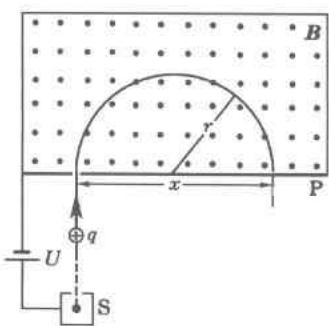
\includegraphics[width=0.2\linewidth]{figures/习题2-43.jpg}
\end{center}

\vfill\newpage

\textbf{2-44.} 如上题, 以钠离子做实验, 得到数据如下: 加速电压 $U = 705 \mathrm{~V}$ , 磁感应强度 $B = 3580 \mathrm{Gs}, x = 10 \mathrm{~cm}$ . 求钠离子的荷质比 $q / m$ .

\vfill


\textbf{2-45.} 一回旋加速器D形电极周围的最大半径 $R = 60\mathrm{cm}$ ，用它来加速质量为 $1.67\times 10^{-27}\mathrm{kg}$ 、电荷为 $1.6\times 10^{-19}\mathrm{C}$ 的质子，要把质子从静止加速到 $4.0\mathrm{MeV}$ 的能量。

(1) 求所需的磁感应强度 B;

(2) 设两 D 形电极间的距离为 1.0 cm，电压为 $2.0 \times 10^{4} V$ ，其间电场是均匀的，求加速到上述能量所需的时间。

\vfill\newpage

\textbf{2-46.} 一电子在 $B = 20\mathrm{Gs}$ 的磁场里沿半径 $R = 20\mathrm{cm}$ 的螺旋线运动。螺距 $h = 5.0\mathrm{cm}$ ，如本题图。已知电子的荷质比 $e / m = 1.76 \times 10^{11}\mathrm{C / kg}$ 。求这电子的速度。

\begin{center}
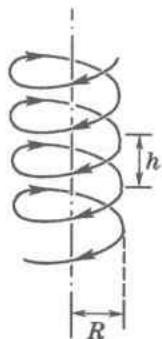
\includegraphics[width=0.15\linewidth]{figures/习题2-46.jpg}
\end{center}

\vfill


\textbf{2-47.} 本题图是微波技术中用的一种磁控管的示意图。一群电子在垂直于磁场 $B$ 的平面内作圆周运动。在运行过程中它们时而接近电极1，时而接近电极2，从而使两电极间的电势差作周期性变化。试证明电压变化的频率为 $eB / 2\pi m$ ，电压的幅度为
$$
U _ {0} = \frac {N e}{4 \pi \varepsilon_ {0}} \left(\frac {1}{r _ {1}} - \frac {1}{r _ {1} + D}\right),
$$
式中 $e$ 是电子电荷的绝对值，$m$ 是电子的质量，$D$ 是圆形轨道的直径，$r_{1}$ 是电子群最靠近某一电极时的距离，$N$ 是这群电子的数目。
\begin{center}
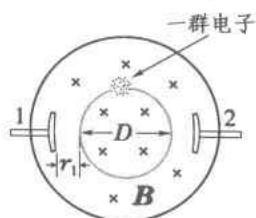
\includegraphics[width=0.3\linewidth]{figures/习题2-47.jpg}
\end{center}


\vfill\newpage

\textbf{2-48.} 在空间有互相垂直的均匀电场 $\pmb{E}$ 和均匀磁场 $\pmb{B},\pmb{B}$ 沿 $x$ 方向， $\pmb{E}$ 沿 $z$ 方向，一电子开始时以速度 $\pmb{v}$ 沿 $y$ 方向前进（见本题图），问电子运动的轨迹如何？

\begin{center}
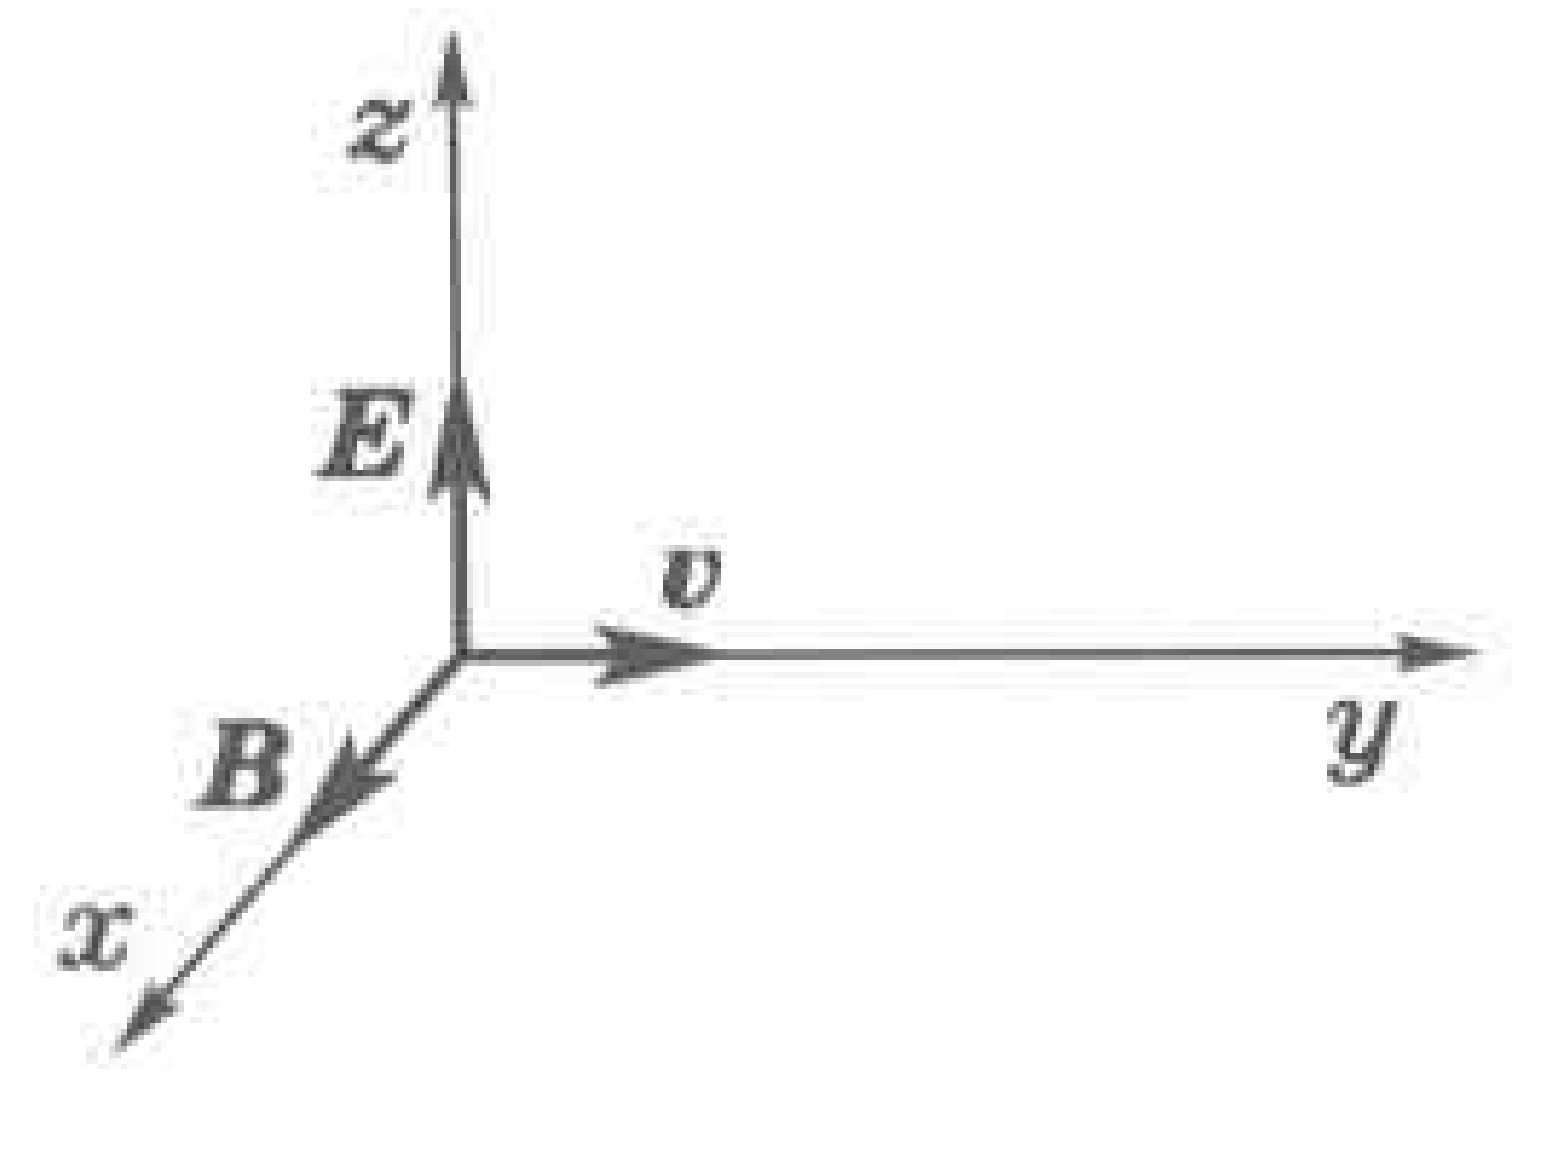
\includegraphics[width=0.3\linewidth]{figures/习题2-48.jpg}
\end{center}

\vfill


\textbf{2-49.} 一铜片厚为 $d = 1.0\mathrm{mm}$ ，放在 $B = 1.5\mathrm{T}$ 的磁场中，磁场方向与铜片表面垂直（见本题图）。已知铜片里每立方厘米有 $8.4\times 10^{22}$ 个自由电子，每个电子电荷的大小为 $e = 1.6\times 10^{-19}\mathrm{C}$ ，当铜片中有 $I = 200\mathrm{A}$ 的电流时，

(1) 求铜片两边的电势差 $U_{aa'}$ ;

(2) 铜片宽度 b 对 $U_{aa}$ 有无影响？为什么？
\begin{center}
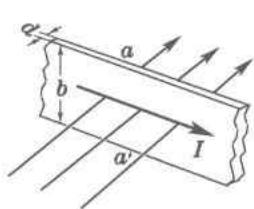
\includegraphics[width=0.3\linewidth]{figures/习题2-49.jpg}
\end{center}

\vfill\newpage

\textbf{2-50.} 一块半导体样品的体积为 $a \times b \times c$ ，如本题图所示，沿 $x$ 方向有电流 $I$ ，在 $z$ 轴方向加有均匀磁场 $B$ . 实验数据为 $a = 0.10 \mathrm{~cm}, b = 0.35 \mathrm{~cm}, c = 1.0 \mathrm{~cm}, I = 1.0 \mathrm{~mA}, B = 3000 \mathrm{Gs}$ ，片两侧的电势差 $U_{\mathrm{AA}'} = 6.55 \mathrm{mV}$ .

(1) 问这半导体是正电荷导电(P型)还是负电荷导电(N型)?

(2) 求载流子浓度(即单位体积内参加导电的带电粒子数)。
\begin{center}
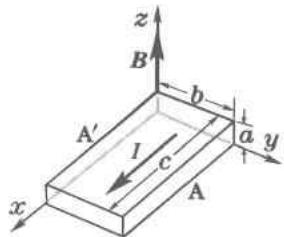
\includegraphics[width=0.3\linewidth]{figures/习题2-50.jpg}
\end{center}
\vfill
\newpage